\documentclass[10pt,a4paper]{article}
\usepackage[margin=20mm]{geometry}
\usepackage[T1]{fontenc}
\usepackage{lmodern}
\usepackage{amsmath,amssymb,booktabs,array,graphicx,enumitem,hyperref}
\hypersetup{colorlinks=true,urlcolor=blue,citecolor=blue,linkcolor=blue}
\setlength{\parindent}{0pt}
\setlength{\parskip}{5pt}
\setlist{nosep,leftmargin=1.5em}
\renewcommand{\arraystretch}{1.13}
% Replace this line when the three team members provide names and student IDs.
\newcommand{\TeamAuthors}{Team member names and student IDs to be supplied}

% Generated from audited results; do not edit numeric values manually.
\newcommand{\DefaultReturn}{\ensuremath{-1.417 \pm 0.044}}
\newcommand{\DefaultCVR}{\ensuremath{0.068 \pm 0.025}}
\newcommand{\DefaultEnergy}{\ensuremath{13.989 \pm 0.432}}
\newcommand{\ThermostatEnergy}{14.939}
\newcommand{\ThermostatCVR}{0.010}
\newcommand{\AbstractFinding}{The highest observed mean PPO return is -1.377 for lambda=0.99; rankings are descriptive given only three training seeds.}
\newcommand{\LearningFinding}{Across the default runs, mean validation return changes from -839.501 before training to -1.551 at the final budget. The strongest mean validation point is -1.365; its difference from the final point is retained by the evaluation protocol. Thus a longer budget does not justify assuming that every run's final policy is its best policy.}
\newcommand{\PerformanceFinding}{The default uses 6.4 percent less electricity than the thermostat reference. Its CVR is 0.058 percentage points higher. Among PPO configurations, lambda=0.99 has the highest observed mean return (-1.377), with 0.056 percent CVR and 13.608 kWh. This is an observed grid ranking, not a test-based choice used to retrain or select checkpoints.}
\newcommand{\ClipFinding}{Mean final-test returns for clip ranges 0.1, 0.2, and 0.3 are -1.508, -1.417, -1.929, respectively. Corresponding mean update KL estimates are 0.002838, 0.008136, 0.0245. The largest clip's weakest seed is 2, at -2.866; this run is retained in all summaries. Relative to the same seed labels at the default, clip=0.1 improves return in 0 of 3 pairs (mean difference -0.091). These diagnostics describe realized updates and do not establish a hard trust-region constraint.}
\newcommand{\LambdaFinding}{At lambda 0.90, 0.95, and 0.99, mean final-test returns are -1.501, -1.417, -1.377. Across-seed return standard deviations are 0.162, 0.044, 0.030. Relative to the same seed labels at the default, lambda=0.99 improves return in 3 of 3 pairs (mean difference +0.040). This changes the advantage estimator at fixed gamma; its ranking should not be extrapolated to every thermal timescale or value-function accuracy.}
\newcommand{\EpochFinding}{Five, ten, and twenty epochs give final-test returns of -1.447, -1.417, -1.441. The corresponding optimization counts are 40,000, 80,000, and 160,000 mini-batch steps. Default has the highest observed mean return within this slice; additional optimization is not intrinsically a guarantee of better closed-loop control.}
\newcommand{\StabilityFinding}{The default's mean late-validation standard deviation is 0.160. The largest mean late peak-to-final drop occurs for Default (0.195 return units).}
\newcommand{\RuntimeFinding}{Mean training wall times excluding periodic validation are 113.3 seconds, 129.4 seconds, 194.5 seconds for 5, 10, and 20 epochs, respectively.}
\newcommand{\ConclusionFinding}{Within the frozen seven-configuration experiment, lambda=0.99 achieves the highest observed mean final-test return. The default's physical outcomes are 0.068 percent CVR, 0.018 degree-hours, and 13.989 kWh per seven-day episode. Relative to the thermostat, it uses 6.4 percent less electricity; the comfort comparison must be considered separately. The principal result is a task-specific account of sample efficiency, comfort--energy balance, update variability, and computational cost, rather than a universal optimal PPO setting.}
\newcommand{\CoverageFinding}{The finite tables have unequal weather-offset coverage (validation versus test, degrees C): hot: [-1.75, -0.94] versus [-1.78, 1.11]; transition: [-1.82, -0.44] versus [-1.57, 1.91]. These conditions remain within training support, but validation rankings need not match test rankings. In particular, the largest-clip run with seed 2 has appreciably worse final-test control in some hot and transition conditions. An independent model reload reproduces its test metrics exactly; it is retained without retuning the protocol.}
\newcommand{\TrajectoryFinding}{For these fixed cold, hot, and transition examples, the default PPO's median indoor temperatures are 21.02, 24.88, 21.84 degrees C, respectively. The comfort bands and thermostat setpoints supply context for where the learned controller operates. Cumulative electricity is monotone and ends at the episode energy; temperature boundary crossings and action changes should be interpreted jointly rather than equated with instability on their own.}
\newcommand{\SlidePerformance}{Default: 0.07 percent CVR, 13.99 kWh; thermostat: 0.01 percent, 14.94 kWh.}
\newcommand{\SlideClip}{Mean return, small/default/large: -1.508, -1.417, -1.929.}
\newcommand{\SlideLambda}{Mean return, small/default/large: -1.501, -1.417, -1.377.}
\newcommand{\SlideEpochs}{Mean training time, 5/10/20 epochs: 113/129/195 seconds.}
\newcommand{\SlideStability}{Largest mean late-validation peak-to-final drop: Default, 0.19 return units.}
\newcommand{\SlideConclusion}{Highest observed mean PPO return: lambda=0.99 (-1.377); this is a descriptive grid result.}

\newcommand{\fig}[3]{\begin{center}\includegraphics[width=#2\linewidth]{../results/figures/#1.pdf}\par{\small\textbf{Figure #3.} \csname Caption#1\endcsname}\end{center}}
\newcommand{\Captionlearningcurves}{Validation returns across training seeds. Shading denotes one sample standard deviation. The bottom row enlarges the period after 102,400 steps.}
\begin{document}
\begin{center}
{\LARGE\bfseries PPO Hyperparameters for Single-Room HVAC Control}\par
\vspace{3mm}
{\large Clipping, GAE Lambda, and Update Epochs}\par
\vspace{3mm}
AIAA 5034, Fall 2026 --- Topic 16\par
\TeamAuthors
\end{center}

\section*{Abstract}
We study how three proximal policy optimization (PPO) hyperparameters affect the control of a synthetic single-room heating, ventilation, and air-conditioning (HVAC) model. The simulator uses two lumped thermal states, a continuous heating/cooling action, and a reward combining temperature discomfort and electricity use. We pre-register a one-factor-at-a-time comparison of clip range, generalized advantage estimation (GAE) lambda, and optimization epochs: seven configurations, three training seeds each, and 512,000 environment interactions per run. Validation and final test conditions are fixed and disjoint. On the final test set, the default PPO obtains a return of \DefaultReturn{}, a comfort violation rate of \DefaultCVR{}\%, and \DefaultEnergy{} kWh per seven-day episode (means across training seeds). The thermostat reference consumes \ThermostatEnergy{} kWh with \ThermostatCVR{}\% violations. \AbstractFinding{} The results characterize comfort--energy trade-offs, learning trajectories, and update stability rather than establishing a universal parameter setting. All experiments run locally on an Apple M4 CPU.

\section*{1. Problem and research questions}
Building temperature control requires decisions whose consequences persist through stored heat. Heating or cooling improves comfort but consumes electricity; allowing temperature to drift reduces immediate energy use but can increase later discomfort. A policy therefore needs a consistent objective and information about both the indoor air and the building's slower thermal response.

This project addresses the course requirement to train PPO on a simple room model and ablate its clip range, GAE lambda, and number of epochs. We ask:
\begin{enumerate}
\item How do these parameters affect learning progress at an equal environment-interaction budget?
\item Which changes in comfort, electricity use, and variability remain visible across independent training seeds?
\item Do update diagnostics help explain the observed learning behavior and computational cost?
\end{enumerate}

The room simulator, physical checks, and metric functions were supplied by a teammate before this study. We add reproducible training, common evaluation for learned and rule-based controllers, the controlled experiment, and an auditable analysis. The environment is kept fixed throughout the ablation.

\subsection*{Scope of the conclusions}
We study the supplied synthetic environment, not a calibrated real building. Energy is an actuator electricity proxy based on constant coefficient of performance (COP). The room does not model humidity, infiltration, occupancy uncertainty, or detailed equipment cycling. These simplifications make the experiment small enough for systematic local training, while bounding what can be inferred about actual HVAC operation.
\clearpage

\section*{2. Background and thermal modeling}
PPO uses on-policy trajectories and a clipped surrogate objective to discourage excessively large policy changes during repeated optimization of the same data~\cite{ppo}. GAE combines temporal-difference residuals over multiple horizons and exposes a bias--variance parameter, lambda~\cite{gae}. These mechanisms act at different stages: GAE changes the learning signal, clipping changes the policy objective, and epochs change how extensively a rollout is optimized. Their effects need not be monotonic or independent of the task.

We use Stable-Baselines3 (SB3), an established PyTorch implementation~\cite{sb3}, rather than introducing another PPO implementation as a confound. The experiment adds observation, evaluation, and artifact-management hooks around the algorithm. Physical trajectories and unnormalized metrics are evaluated independently of the training wrapper.

Resistor--capacitor (RC) networks offer a compact representation of building heat dynamics. Bacher and Madsen discuss model structures including indoor/envelope nodes~\cite{bacher}; the delivered environment adopts a two-node topology and synthetic-case parameters documented from Zamani et al.~\cite{zamani}. The comfort ranges follow the office evaluation ranges cited in the teammate's modeling notes~\cite{hvacreview}; their mapping to the three synthetic weather classes is a project assumption.

\subsection*{Two-node heat balance}
Let $T_i$ be the indoor equivalent temperature and $T_e$ the envelope equivalent temperature. Outdoor temperature $T_o$ is an exogenous forcing. With time measured in hours and thermal powers in kW,
\begin{align}
C_i\dot T_i &= (T_e-T_i)/R_{ie}+Q_{\mathrm{hvac}}+Q_g,\\
C_e\dot T_e &= (T_o-T_e)/R_{eo}+(T_i-T_e)/R_{ie}.
\end{align}
Heat flows down temperature gradients, with thermal resistance setting the flow magnitude. Capacitance converts net heat input into a temperature rate, representing storage and inertia. Internal indoor/envelope exchange cancels when the two energy balances are added.

\begin{center}
\begin{tabular}{lll}
\toprule Parameter & Value & Meaning \\
\midrule
$R_{ie}$ & 27.81 $^\circ$C/kW & Indoor--envelope resistance \\
$R_{eo}$ & 3.02 $^\circ$C/kW & Envelope--outdoor resistance \\
$C_i$ & 1.11 kWh/$^\circ$C & Indoor equivalent capacitance \\
$C_e$ & 2.11 kWh/$^\circ$C & Envelope equivalent capacitance \\
Heating/cooling capacity & 1 kW each & Maximum thermal power \\
Heating/cooling COP & 3 each & Thermal power / electric power \\
Control interval & 0.25 h & 96 control decisions per day \\
\bottomrule
\end{tabular}
\end{center}

The continuous system is linear in its state and inputs. At construction, a zero-order-hold discretization gives $x_{t+1}=A_dx_t+B_dv_t$, with $x=[T_i,T_e]^\top$ and $v=[Q_{\mathrm{hvac}},Q_g,T_o]^\top$. Each forcing and action is held constant within the interval. This avoids repeated numerical integration during learning.

The delivered test suite checks continuous energy balance, steady states, passive decay, actuator direction, and agreement with an independent ODE solution. All 76 existing tests pass on the Mac. These are implementation checks, not validation against measured building temperatures.
\clearpage

\section*{3. Environment, observations, and objective}
\subsection*{Observation and action}
The controller receives an 11-dimensional observation through a Gymnasium interface. Only $T_i$ and $T_e$ are dynamic thermal states; the other entries describe boundary conditions, targets, and phase.

\begin{center}
\begin{tabular}{clp{88mm}}
\toprule Indices & Entries & Interpretation \\
\midrule
0--1 & $T_i,T_e$ & Indoor and envelope temperatures, $^\circ$C \\
2 & $T_o$ & Outdoor temperature, $^\circ$C \\
3 & $Q_g$ & Internal heat gain, thermal kW \\
4--5 & $L,U$ & Lower/upper comfort bounds, $^\circ$C \\
6--7 & $\sin(2\pi h/24),\cos(2\pi h/24)$ & Daily phase without a midnight discontinuity \\
8--10 & Weather one-hot code & Cold, hot, transition class \\
\bottomrule
\end{tabular}
\end{center}

The action $u\in[-1,1]$ sets heating ($u>0$), cooling ($u<0$), or off ($u=0$). With the symmetric default capacity, $Q_{\mathrm{hvac}}=u$ thermal kW. Electric power is $|u|/3$ kW, so each interval uses $E_t=|u_t|\Delta t/3$ kWh. SB3 samples an unsquashed Gaussian action during training and clips the executed action to the environment bounds. All configurations retain the same action handling.

\subsection*{Weather, gains, and resets}
The outdoor forcing is $T_o(h)=\mu+\delta+A\sin(2\pi(h-9)/24)$. Temperature peaks at 15:00. Each training episode samples a weather class uniformly, one offset $\delta\sim U[-2,2]$, and an indoor initial temperature within $\pm2^\circ$C of the comfort midpoint. Initial envelope temperature satisfies its instantaneous zero-net-flow condition. Actual reset values are saved for evaluation.

\begin{center}
\begin{tabular}{lrrl}
\toprule Weather & $\mu$ ($^\circ$C) & $A$ ($^\circ$C) & Comfort interval ($^\circ$C) \\
\midrule Cold & 5 & 6 & [20, 23.5] \\
Hot & 31 & 6 & [23, 26] \\
Transition & 19 & 8 & [20, 23.5] \\
\bottomrule
\end{tabular}
\end{center}

Internal gains combine 0.05 kW continuously, 0.15 kW during 08:00--18:00, and a daytime half-sine peaking at 0.15 kW. Every episode lasts seven days (672 steps); this is a time truncation, not a physical terminal event. SB3 bootstraps at the time limit. Within an episode, the daily forcing repeats.

\subsection*{Reward and physical metrics}
For post-step temperature, $d_t=\max(0,L-T_{i,t+1},T_{i,t+1}-U)$. The fixed reward is
\begin{equation}
r_t=-w_c\Delta t\,d_t-w_e E_t,\qquad w_c=1,\quad w_e=0.1.
\end{equation}
Weights use the numerical values in the specified units. We report electricity $\sum_tE_t$, discomfort $\sum_td_t\Delta t$ in degree-hours, and the comfort violation rate (CVR), $100\,\mathrm{mean}(d_t>10^{-8})$. Thus the raw episode return equals minus degree-hours minus 0.1 times kWh, an identity checked by the evaluator. CVR approximates violation frequency at interval endpoints. Initial observations are plotted but not counted as completed intervals.
\clearpage

\section*{4. PPO and the three studied parameters}
The actor uses two 64-unit Tanh layers to output the Gaussian action mean, together with a learned state-independent log standard deviation. A separate two-layer 64-unit value network estimates future discounted return. Together they have 9,987 parameters. Observations are normalized with running statistics; rewards are not normalized. Validation and test reuse frozen observation statistics and deterministic actions.

\subsection*{GAE lambda: the advantage estimate}
For nonterminal transitions, the temporal-difference residual and GAE are
\begin{align}
\delta_t &= r_t+\gamma V_{\mathrm{old}}(o_{t+1})-V_{\mathrm{old}}(o_t),\\
\hat A_t &= \sum_{l=0}^{L-1}(\gamma\lambda)^l\delta_{t+l}.
\end{align}
Termination masks are omitted for readability. Real terminal states omit the bootstrap term; rollout boundaries and the artificial seven-day limit retain appropriate bootstrap estimates without carrying the recursion across a reset. Smaller lambda relies more on short-horizon bootstrapping. Larger lambda uses longer reward fragments and can increase variance. Gamma is fixed at 0.99 and is distinct from lambda.

\subsection*{Clip range: the policy objective}
PPO maximizes
\begin{equation}
L^{\mathrm{clip}}(\theta)=\mathbb{E}_t\!\left[\min\!\left(\rho_t\hat A_t,
\mathrm{clip}(\rho_t,1-\epsilon,1+\epsilon)\hat A_t\right)\right],
\end{equation}
where $\rho_t=\pi_\theta(a_t\mid o_t)/\pi_{\mathrm{old}}(a_t\mid o_t)$. Positive advantages encourage increased likelihood; negative advantages encourage decreased likelihood. Clipping removes additional objective gains from sufficiently large changes in the encouraged direction. It is not a hard guarantee that all ratios or KL divergences remain within bounds. The baseline distribution is fixed to the policy that collected the rollout.

The value network minimizes a squared error to $\hat R_t=\hat A_t+V_{\mathrm{old}}(o_t)$. The total minimized objective is $-L^{\mathrm{clip}}+0.5L_V-c_H H$, with $c_H=0$ here. Policy gradients differentiate action log probabilities through the neural network, not through the thermal simulator.

\subsection*{Epochs: repeated use of each rollout}
We collect 2,048 steps from one environment, then form shuffled mini-batches of 64. Each epoch has 32 optimizer steps. Five, ten, and twenty epochs therefore give 160, 320, and 640 mini-batch updates per rollout, respectively. At the common budget, these correspond to 40,000, 80,000, and 160,000 optimizer steps. Reuse can improve sample efficiency but also strengthens policy movement and increases computation.

Learning rate is fixed at $3\times10^{-4}$, advantages are normalized, global gradient norm is capped at 0.5, value clipping is disabled, and no target-KL early stopping is applied. These choices are held constant to isolate the specified factors. Their interactions with the studied parameters remain outside this experiment.
\clearpage

\section*{5. Experimental design and reproducibility}
We use a one-factor-at-a-time design around $(\epsilon,\lambda,K)=(0.2,0.95,10)$:
\begin{center}
\begin{tabular}{lrrr}
\toprule Configuration & Clip range & GAE lambda & Epochs \\
\midrule Default & 0.2 & 0.95 & 10 \\
Clip small & 0.1 & 0.95 & 10 \\
Clip large & 0.3 & 0.95 & 10 \\
Lambda small & 0.2 & 0.90 & 10 \\
Lambda large & 0.2 & 0.99 & 10 \\
Epochs few & 0.2 & 0.95 & 5 \\
Epochs many & 0.2 & 0.95 & 20 \\
\bottomrule
\end{tabular}
\end{center}
Sharing the default yields seven configurations. Seeds 0, 1, and 2 give 21 independent runs, each with 512,000 interactions and 250 rollouts. Total training interaction count is 10,752,000, excluding evaluation. This design estimates local single-factor effects, not all parameter interactions.

\subsection*{Pilot and protocol freeze}
Before final testing, a 102,400-step default pilot reached a validation return of $-1.496$ from approximately $-840.040$, and CVR decreased from 72.66\% to 0.06\%. Its learning wall time was 29.0 seconds. This supported using the implementation and a five-times-longer fixed budget for the comparison; it did not establish convergence. The protocol was committed before formal execution. No final test feedback was used to set the budget.

\subsection*{Validation, test, and references}
The fixed validation table contains five conditions per weather class (15 total). A separate table contains ten per class for final testing (30 total), with no repeated physical condition across the two splits. Each stores weather offset, both initial temperatures, and a reset seed. Training conditions continue to be sampled from the original distribution. The test set is in-distribution and does not establish robustness to unseen building parameters or real weather.

Validation occurs after complete updates every 20,480 samples. The final model at exactly 512,000 steps is tested, regardless of its best earlier validation score. All methods see the same test conditions. References are (i) HVAC off and (ii) a full-power relay controller targeting the comfort midpoint with a $\pm0.5^\circ$C deadband. The latter is a useful conventional controller, not an oracle optimized for this reward.

We first average conditions within each trained model, then report the mean and sample standard deviation across the three training seeds. Weather classes are equally weighted. Thirty test episodes from one model are not thirty independent training repetitions. We use descriptive comparisons without significance claims.

\subsection*{Local execution and audit trail}
Experiments run in the Conda environment \texttt{ppo} on an M4 MacBook Air with 16 GB memory. Two independent processes run under \texttt{screen}, each using one PyTorch thread. SB3 2.7.0, PyTorch 2.8.0, Gymnasium 1.2.3, NumPy 2.2.6, and SciPy 1.15.3 are recorded. Each run saves configuration, source hash, Git commit, dependency versions, model, normalizer, evaluation traces, and artifact checksums. Complete runs are skipped only after integrity checks. The pipeline has 86 passing environment and integration tests before formal execution.
\clearpage

\section*{6. Learning progress at a fixed sample budget}
\begin{center}
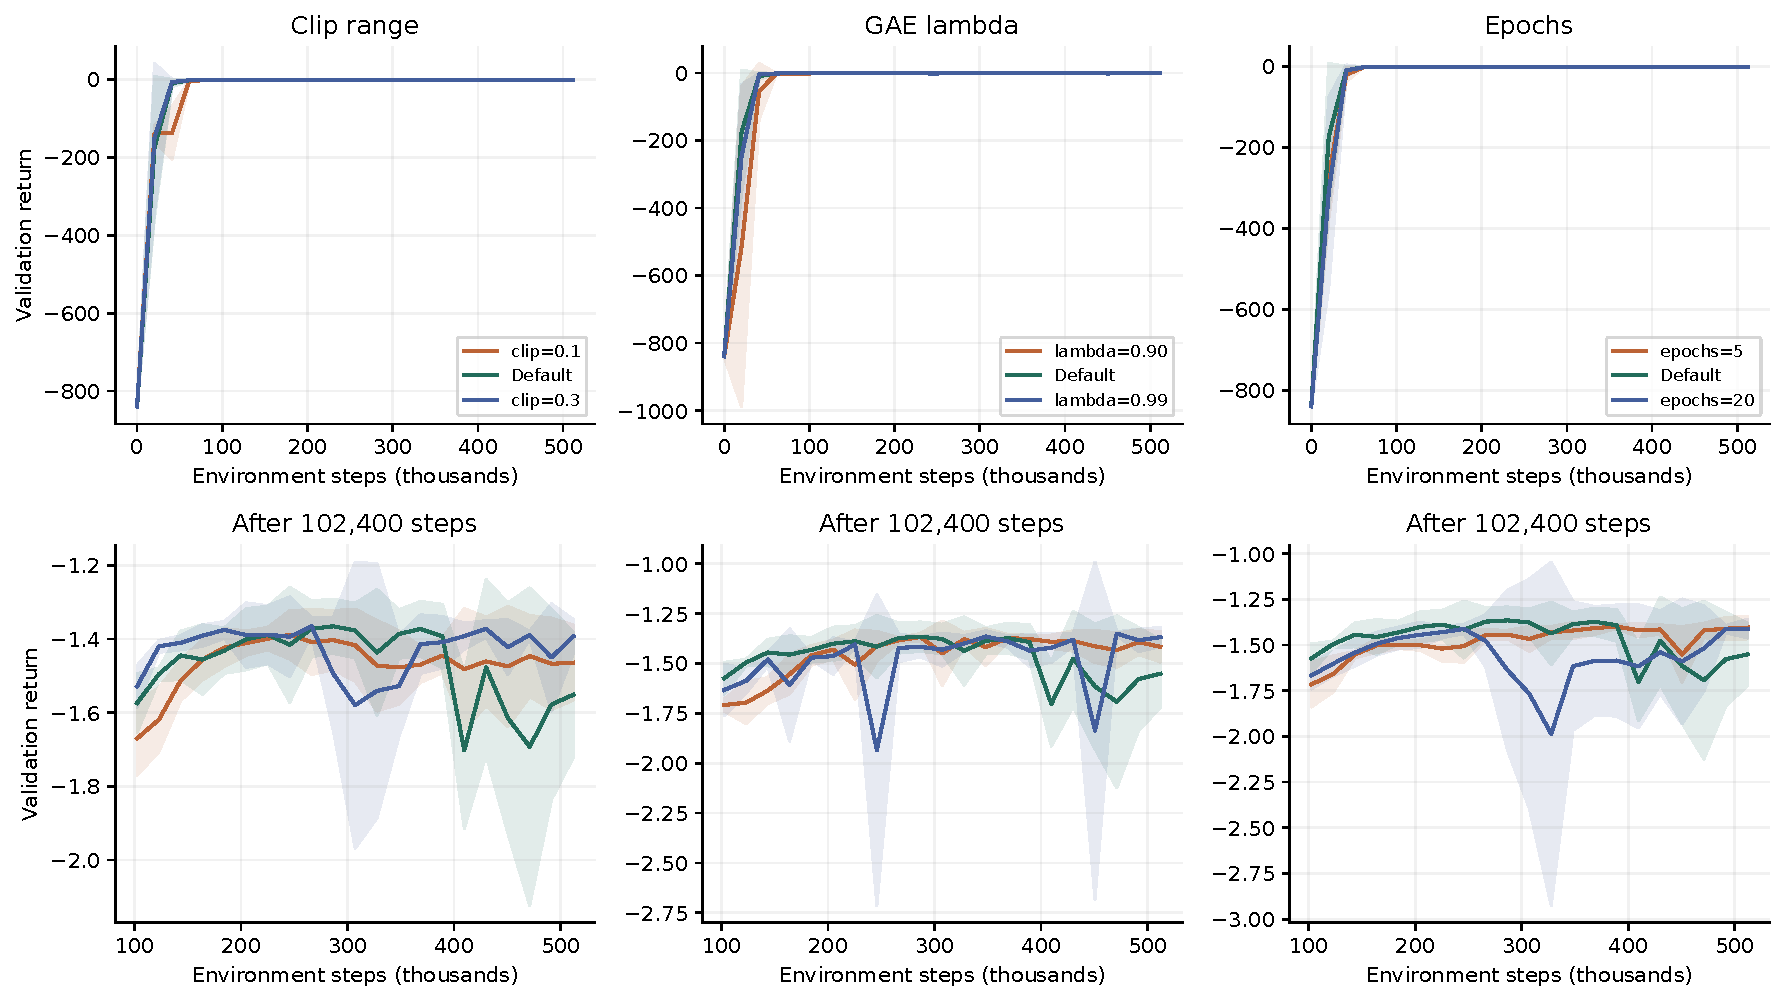
\includegraphics[width=\linewidth]{../results/figures/learning_curves.pdf}\par
{\small\textbf{Figure 1.} Validation return, mean and one sample standard deviation across three training seeds. Bottom panels show the period after 102,400 interactions. The validation set and evaluation rule are common to all runs.}
\end{center}

Higher return means a smaller weighted discomfort--energy penalty. Early changes are dominated by avoiding large temperature deviations; later changes can reflect finer energy control, residual violations, or deterioration. The lower panels prevent the large initial penalties from hiding late differences.

\LearningFinding{}

These trajectories should not be read as guaranteed monotonic improvement. PPO optimizes a sampled clipped objective while the state distribution and advantage estimates evolve. A later update can reduce deterministic validation performance even when the current optimization loss improves. The fixed final-checkpoint rule exposes this behavior rather than selecting each run's best point retrospectively.

The shaded bands quantify only variation among the three training seeds on the same fixed validation conditions. They are not confidence intervals for all buildings or weather distributions. Moreover, validation return combines two physical quantities, so a similar curve can correspond to different comfort and electricity outcomes. The final physical metrics are therefore examined separately.
\clearpage

\section*{7. Final comfort--energy performance}
\begin{center}
{\small
\begin{tabular}{lrrrr}
\toprule Controller & Return & CVR (\%) & Degree-hours & kWh \\
\midrule
HVAC off & -873.775 & 80.724 & 873.775 & 0.000 \\
Thermostat & -1.497 & 0.010 & 0.003 & 14.939 \\
\midrule
Default & \ensuremath{-1.417 \pm 0.044} & \ensuremath{0.068 \pm 0.025} & \ensuremath{0.018 \pm 0.006} & \ensuremath{13.989 \pm 0.432} \\
clip=0.1 & \ensuremath{-1.508 \pm 0.052} & \ensuremath{1.548 \pm 0.241} & \ensuremath{0.132 \pm 0.056} & \ensuremath{13.760 \pm 0.141} \\
clip=0.3 & \ensuremath{-1.929 \pm 0.814} & \ensuremath{3.290 \pm 4.852} & \ensuremath{0.553 \pm 0.862} & \ensuremath{13.761 \pm 0.519} \\
lambda=0.90 & \ensuremath{-1.501 \pm 0.162} & \ensuremath{0.732 \pm 1.174} & \ensuremath{0.106 \pm 0.159} & \ensuremath{13.946 \pm 0.557} \\
lambda=0.99 & \ensuremath{-1.377 \pm 0.030} & \ensuremath{0.056 \pm 0.003} & \ensuremath{0.016 \pm 0.002} & \ensuremath{13.608 \pm 0.283} \\
epochs=5 & \ensuremath{-1.447 \pm 0.052} & \ensuremath{0.193 \pm 0.228} & \ensuremath{0.021 \pm 0.004} & \ensuremath{14.262 \pm 0.521} \\
epochs=20 & \ensuremath{-1.441 \pm 0.046} & \ensuremath{0.053 \pm 0.008} & \ensuremath{0.015 \pm 0.002} & \ensuremath{14.263 \pm 0.462} \\
\bottomrule
\end{tabular}
}
\par
{\small\textbf{Table 1.} Seven-day final-test metrics. PPO entries are mean $\pm$ sample standard deviation across three training seeds after averaging the 30 fixed conditions. Rules are deterministic references, so no training-seed standard deviation is assigned.}
\end{center}

\begin{center}
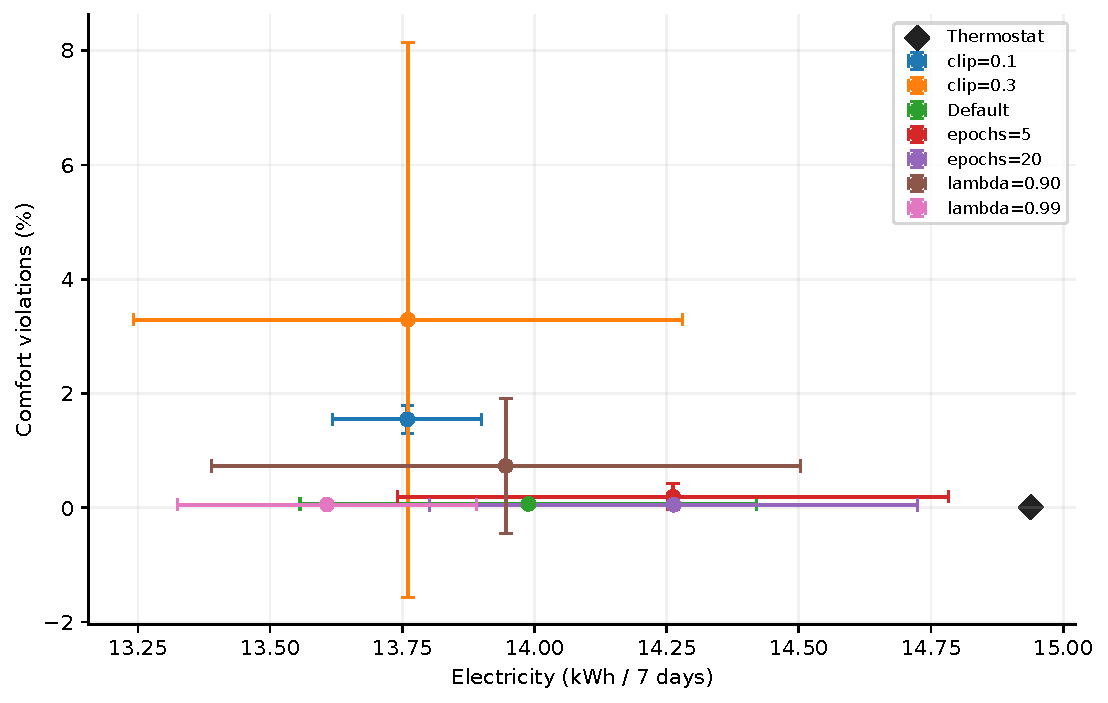
\includegraphics[width=0.85\linewidth]{../results/figures/comfort_energy_tradeoff.pdf}\par
{\small\textbf{Figure 2.} Final-test electricity and CVR. PPO error bars show across-training-seed standard deviations. HVAC off is omitted from this zoomed plot and remains in Table 1.}
\end{center}

\PerformanceFinding{}

The weighted return can prefer a small increase in discomfort if it saves sufficient electricity. Conversely, a low-CVR controller may consume more energy. We therefore avoid interpreting a higher return as automatic improvement in both comfort and electricity. Degree-hours additionally distinguishes frequent tiny boundary crossings from larger deviations.
\clearpage

\section*{8. Hyperparameter effects and update stability}
\begin{center}
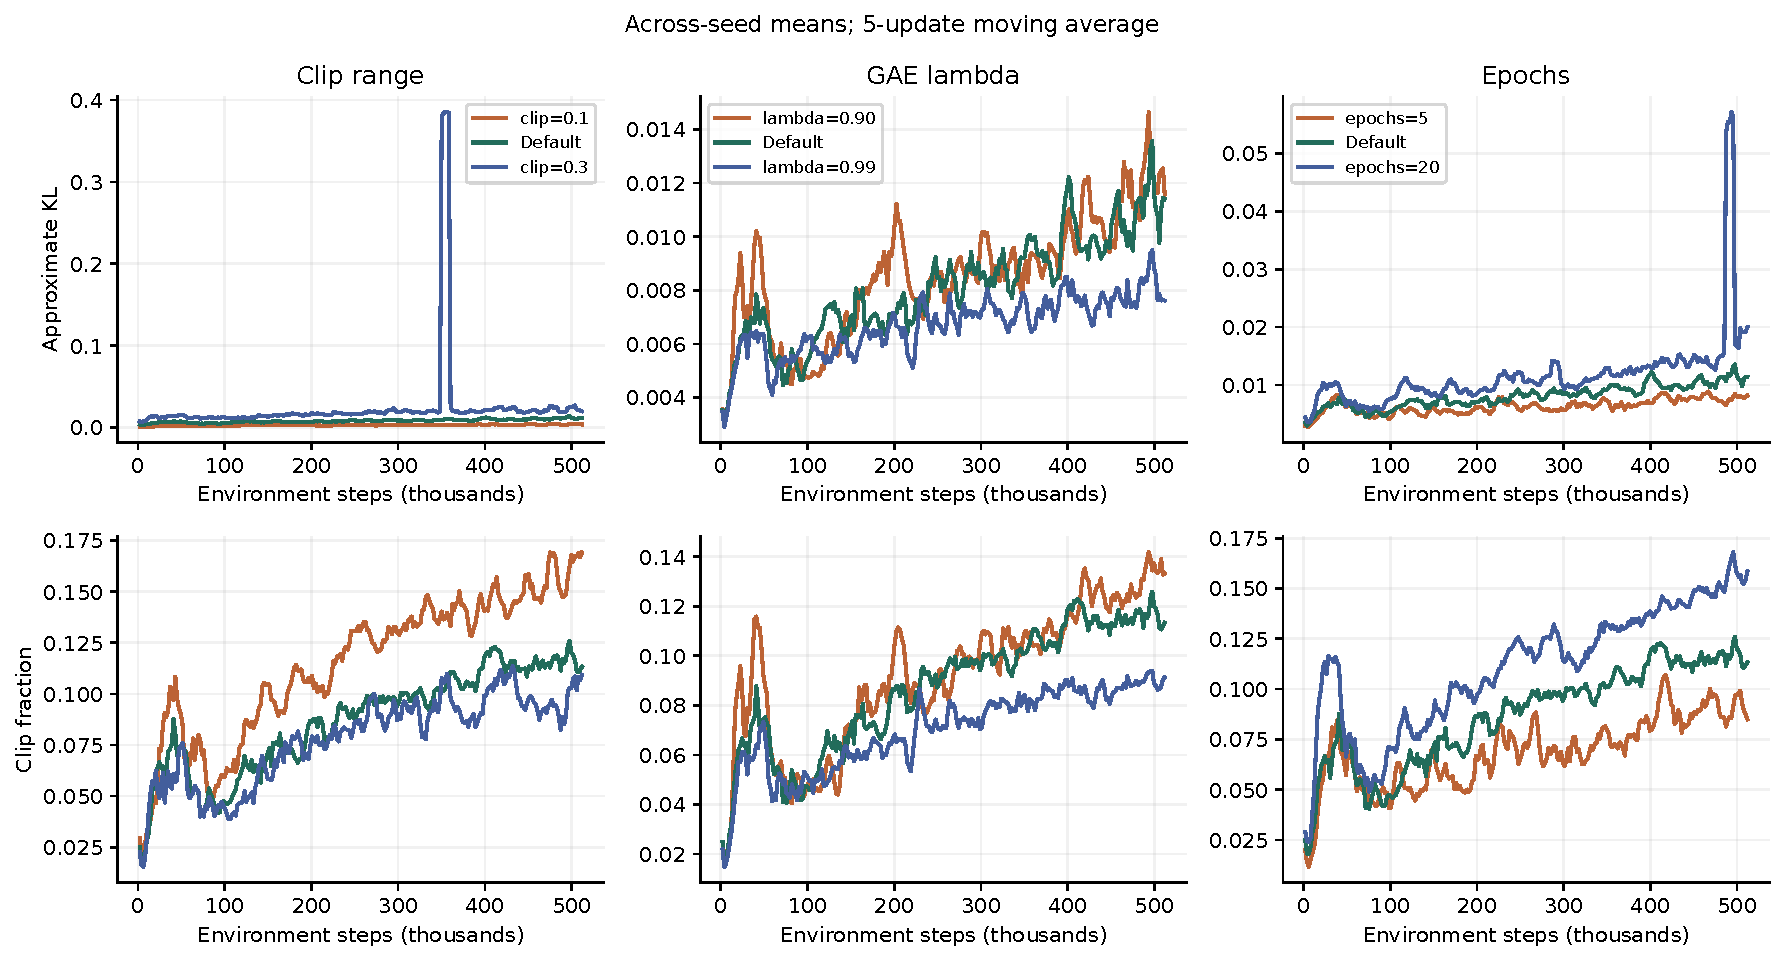
\includegraphics[width=\linewidth]{../results/figures/update_diagnostics.pdf}\par
{\small\textbf{Figure 3.} Approximate KL and clipped-sample fraction. Curves are across-seed means with a five-update moving average; raw per-update data are retained. These diagnostics help characterize changes but do not independently prove stability.}
\end{center}

\textbf{Clip range.} \ClipFinding{}

\textbf{GAE lambda.} \LambdaFinding{}

\textbf{Epochs.} \EpochFinding{}

We also measure late-validation variability over the second half of training and the drop from that interval's peak to the final validation return. \StabilityFinding{} These are descriptive update-sensitivity measures, not replacements for final test metrics or repeated seeds.

The diagnostics and performance rankings need not agree perfectly. A small KL can accompany slow learning, and a high clipping fraction alone does not establish failure. At the same time, the fixed interaction budget entails different computation for different epoch counts. \RuntimeFinding{} Parallel execution, thermal throttling, and other Mac activity can affect wall-clock values; they are practical costs rather than controlled hardware benchmarks.
\clearpage

\section*{9. Representative closed-loop behavior}
\begin{center}
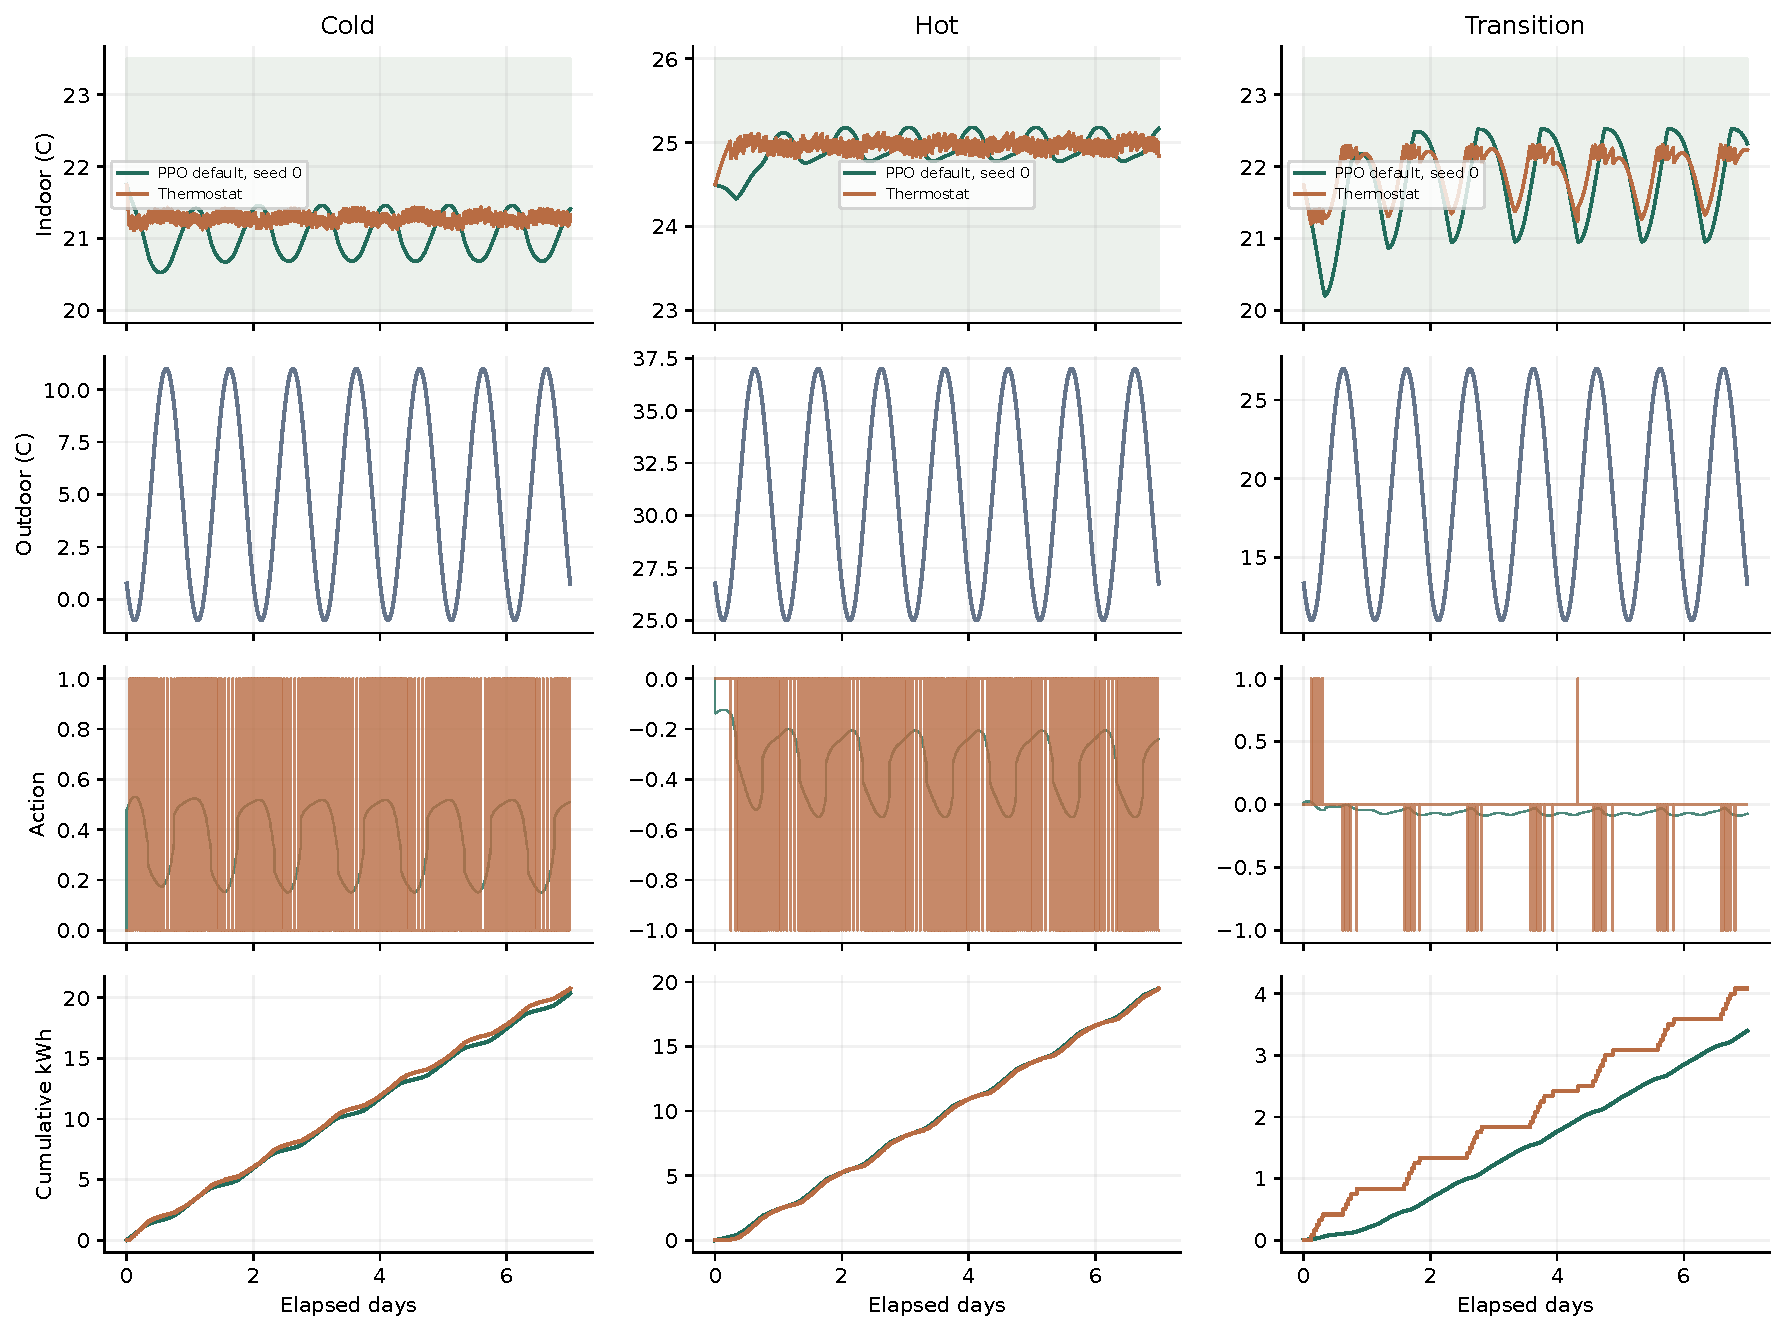
\includegraphics[width=\linewidth]{../results/figures/representative_trajectories.pdf}\par
{\small\textbf{Figure 4.} Preselected test condition 00 for each weather class. Default PPO uses training seed 0; the thermostat uses identical physical conditions. Rows show indoor temperature with the comfort band, outdoor forcing, executed action, and cumulative electricity. Initial points are plotted but excluded from interval metrics.}
\end{center}

\TrajectoryFinding{}

The action is delivered thermal power, not a target temperature. Repeated small heating/cooling commands and periods of inactivity affect both the thermal state and electricity. The envelope state continues to exchange heat after the actuator changes, explaining why immediate reward alone cannot describe all consequences of a decision.

These trajectories are illustrative, with conditions and training seed specified before final analysis. They are not a search for each method's most favorable episode. Population-level conclusions rely on the full fixed test table and all three training seeds, including any seed with poorer control.
\clearpage

\section*{10. Discussion, limitations, and conclusion}
\ConclusionFinding{}

Several qualifications bound this conclusion. Only three training seeds and three candidate values per factor are studied. The one-factor design cannot resolve all interactions with learning rate, gamma, architecture, normalization, or other factors. The two-state model exposes envelope temperature directly and repeats deterministic daily forcing; it omits humidity, ventilation, sensor noise, equipment cycling, and real-world calibration. Constant COP gives an electricity proxy rather than a full building meter prediction. In particular, the selected capacities and gains make this a small synthetic control problem.

The fixed test set provides paired, reproducible conditions, but no out-of-distribution building or climate evaluation. The final-checkpoint rule prevents favorable checkpoint selection, while also allowing a configuration that learned useful control earlier to finish worse. Such deterioration is part of the observed stability result. Three-seed rankings should be interpreted descriptively, not as universal optimal settings or statistically established superiority.

The practical outcome is a complete local workflow: a validated thermal environment, shared physical evaluation, audited PPO runs, controlled ablations, and result generation. An appropriate next extension would add more training seeds or test a small interaction grid while preserving a separate test protocol. Real-building claims would additionally require calibrated dynamics, measurable observations, and representative weather/equipment data.

\begin{thebibliography}{9}
\setlength{\itemsep}{2pt}
\bibitem{ppo} J. Schulman et al. Proximal Policy Optimization Algorithms. arXiv:1707.06347, 2017.
\bibitem{gae} J. Schulman et al. High-Dimensional Continuous Control Using Generalized Advantage Estimation. ICLR, 2016. arXiv:1506.02438.
\bibitem{sb3} A. Raffin et al. Stable-Baselines3: Reliable Reinforcement Learning Implementations. JMLR, 22(268):1--8, 2021.
\bibitem{bacher} P. Bacher and H. Madsen. Identifying suitable models for the heat dynamics of buildings. Energy and Buildings, 43(7):1511--1522, 2011.
\bibitem{zamani} V. Zamani et al. Heating and cooling supply estimation to control buildings temperature using resistor-capacitor thermal model, unscented Kalman filter, and nonlinear least square method. Building Services Engineering Research and Technology, 45(2):135--160, 2024.
\bibitem{hvacreview} A. Manjavacas et al. An experimental evaluation of deep reinforcement learning algorithms for HVAC control. Artificial Intelligence Review, 57:173, 2024.
\bibitem{gym} Farama Foundation. Gymnasium documentation: Env, custom environments, and environment checker. \url{https://gymnasium.farama.org/}.
\end{thebibliography}
\end{document}
